\chapter{Clases y Objetos}
\label{objects}
\index{object}
\index{class}

A esta altura ya sabes cómo usar funciones para organizar código
y tipos integrados para organizar datos. El siguiente paso es aprender
``programación orientada a objetos,`` la cual usa tipos definidos por
el programador para organizar código y datos.
\index{abstraction}
\index{encapsulation}

Cuando las aplicaciones de software comienzan a crecer, el número
de detalles que se debe manejar puede volverse agobiante. La única 
manera de manejar esta complejidad es usar abstracción y encapsulamiento.
La programación orientada a objetos es una manera muy popular y eficiente
de implementar abstracción y encapsulamiento. 

Perl~6 es un {\bf lenguaje de programación orientado a objetos}, lo cual significa
que el lenguaje provee características que soportan la
programación orientada a objetos, la cual posee las siguientes
características definitivas:
\index{object-oriented programming}

\begin{itemize}

\item Los programas incluyen definiciones de clases y métodos.
\index{class}
\index{method}

\item La mayor parte de la computación se expresa en términos de 
operaciones sobre los objetos.

\item Los objetos usualmente representan cosas en el mundo real, y los 
métodos normalmente corresponden a las formas de interacción de las
cosas en el mundo real.
\end{itemize}

La programación orientada a objetos en Perl~6 es un tema enorme que 
merece un libro para sí mismo (y probablemente habrá un libro o dos sobre la
materia en algún punto). Este capítulo hará más que analizar el
tema superficialmente y te permitará crear y usar objetos. Sin embargo,
no cubrirá algunos detalles y características más avanzadas.
\index{OOP (object-oriented programming)}
\index{object-oriented programming (OOP)}

\section{Objetos, Métodos y Programación Orientada a Objetos}
\index{object-oriented programming (OOP)}
\index{programming!object-oriented}

Empecemos con una sinopsis general de la programación orientada a objetos
y una breve introducción a la jerga asociada con la misma.


\index{object}
En la ciencia de la computación, un objeto puede describirse 
vagamente como una dirección de memoria o una entidad que 
posee un valor, y su usualmente es conocido como un identificador.
Esto puede ser una variable, una estructura de datos, un array,
o posiblemente hasta una función. No usaremos esta concepción
general con el mismo sentido en este capítulo.

En la programación orientada a objetos (POO), la palabra
{\bf objeto} tiene un significado mucho más específico: un 
objeto es una identidad que usualmente tiene:
\begin{itemize}

\item Una identidad (por ejemplo, su nombre).

\index{object! behavior}
\item Algunas propiedades que definen su comportamiento (en la forma
de funciones especiales que son comúnmente conocidas como {\bf métodos});
este comportamiento usualmente no cambia con el tiempo y es 
generalmente común a todos los objetos del mismo tipo.
\index{method}

\item Un {\bf estado} el cual es definido por algunas variables
especiales (conocidas como, dependiendo en el lenguaje, atributos,
campos, o miembros); el estado puede cambiar a medida que pasa el 
tiempo y es generalmente específico a cada objeto. En Perl, nos
referimos a dichas variables como {\tt atributos}.
\index{object!state}
\index{object!attribute}
\index{attribute!object}
\end{itemize}

En resumen, un objeto es un conjunto de atributos y métodos
todos juntos.

\index{class}
Los objetos son usualmente definidos dentro de un tipo
de paquete de código conocido como una {\bf clase}. 
Una clase define los métodos y la naturaleza de los
atributos asociados a un objeto. En Perl~6, una clase
hace posible definir nuevos tipos similares a los tipos
integrados que hemos visto hasta ahora. Muy pronto comenzaremos
a definir algunas clases y las usaremos para crear objetos.
\index{type!building new type}

\index{invocant}
\index{method}
\index{dot notation}
Ya sabes informalmente lo qué es un método, dado que hemos
usado métodos integrados a lo largo del libro. Es como una 
como una función con una sintaxis sufija que usa la notación
del punto sobre el invocante. Por ejemplo, puedes invocar el
método {\tt say} sobre una simple cadena de texto:

\begin{lstlisting}
"foo".say;           # -> foo
\end{lstlisting}

Nota que ``foo'' no es un objeto, pero una simple cadena de texto.
No obstante, puedes invocar el método \verb|say| sobre la misma,
debido a que Perl puede tratarla internamente como un objeto cuando
es necesario. En algunos otros lenguajes POO, esta conversión implícita
de un tipo nativo a un objeto es conocida como autoboxing.
\index{autoboxing}

Probablemente recuerdas que los métodos pueden ser encadenados
en un proceso donde el valor devuelto por un método se convierte
en el invocante para el siguiente método:

\begin{lstlisting}
"foo".uc.say;        # -> FOO

my @alfabeto = <charlie foxtrot alpha golf echo bravo delta>;
@alfabeto.sort.uc.say;
    # imprime: ALPHA BRAVO CHARLIE DELTA ECHO FOXTROT GOLF 
\end{lstlisting}

\index{role}
En POO, los métodos que se pueden aplicar a los objetos son
usualmente definidos dentro de las clases, regularmente
la clase que también definió el objeto o alguna otra clase 
con una cercana relación. En Perl~6, los métodos pueden también
ser definidos en un {\bf role}, el cual es otro tipo de 
paquete de código que se parece a una clase, como veremos
más adelante.

\index{black box}
\index{encapsulation}
La idea básica de la programación orientada a objetos es
que un objeto es un tipo de caja negra que oculta su
estructura interna (datos y código) del usuario; el usuario
puede consultar o cambiar el estado de un objeto a través de
los métodos. El proceso de ocultar la estructura interna
de los objetos se conoce como {\bf encapsulación}. Esto usualmente
permite tener una perspectiva más general y una mejor abstracción
de datos con respecto a lo que hemos visto hasta ahora;
esto resulta en programas con menos errores (especialmente programas
extensos).

En adición, POO usualmente ofrece los siguientes conceptos:
\begin{itemize}
\index{polymorphism}
\item {\bf polimorfismo}, i.e., la función o el método tiene la
posibilidad de hacer cosas diferentes dependiendo del tipo de 
objeto que la llama o lo invoca;
\index{inheritance}
\item {\bf herencia}, i.e., la posibilidad de derivar una clase de
otra clase, de tal manera que la clase hija hereda algunas de la 
propiedades de la clase {\bf padre}, la cual es una herramienta
poderosa para el reutilización de código.
\end{itemize}

Ahora estudiaremos cómo todo estos conceptos se implementan en Perl.


\section{Tipos Definidos por el Programador}
\label{point}
\index{programmer-defined type}
\index{type!programmer-defined}

Hemos usado muchos tipos integrados de Perl; ahora vamos
a definir un nuevo tipo. Como un ejemplo, crearemos un
tipo llamado {\tt Punto2D} que representa a un punto en
el espacio bidimensional.
\index{point, mathematical}
\index{two-dimensional space}

En notación matemática, los puntos son usualmente escritos
en paréntesis con una coma que separa las coordenadas.  Por 
ejemplo, en las coordenadas cartesianas o rectangulares,
$(0,0)$ representa el origen, y $(x,y)$ representa un punto
$x$ unidades a la derecha y $y$ unidades a la izquierda. $x$
se llama la abscisa y $y$ la ordenada.
\index{Cartesian coordinates}
\index{coordinates!Cartesian}
\index{coordinates!rectangular}
\index{rectangular coordinates}

Hay varias maneras de representar un punto en Perl:

\begin{itemize}

\item Podemos almacenar las coordenadas separadamente 
en dos variables, {\tt \$x} y {\tt \$y}.

\item De igual manera, podemos almacenar las coordenadas como
elementos en una lista, un array, o una pareja.

\item Así mismo, podemos crear un nuevo tipo que representa
puntos como objetos.

\end{itemize}
\index{representation}

Crear un nuevo tipo es un poco más complicado que las otras
opciones, pero tiene ventajas que serán aparentes muy pronto.

Un tipo definido por el programador es usualmente creado con 
una {\bf clase} (o un {\bf rol}, pero regresaremos a esto más tarde).
La definición de una clase bien simple para un tipo que representa a 
un punto luce así:
\index{class}
\index{object!class}
\index{class!definition}
\index{definition!class}
\index{role}
\index{Point2D class}

\begin{lstlisting}
class Punto2D {
    has $.abscisa;               # valor "x"
    has $.ordenada;              # valor "y" 
}
\end{lstlisting}
%
La cabecera indica que la nueva clase se llama {\tt Punto2D}. 
El cuerpo define dos atributos, i.e., propiedades con nombres
asociadas con la clase, aquí la abscisa y la ordenada 
(o las coordenadas $x$ y $y$) del punto.
\index{Point2D class}
\index{class!Point2D}

\index{type object}
La definición de una clase con el nombre {\tt Punto2D} crea
un {\bf tipo objeto}.

El tipo objeto es como una factoría para crear objetos. Para crear
un punto, tú llamas el método {\tt new} sobre la clase {\tt Punto2D}:

\begin{lstlisting}
my $punto = Punto2D.new( 
    abscisa  => 3, 
    ordenada => 4
);
say $punto.WHAT;                # -> (Point2D)
say $punto.isa(Punto2D)         # -> True
say $punto.abscisa;             # -> 3
\end{lstlisting}
%
\index{isa method}
\index{WHAT}
Por supuesto puedes crear tanto puntos como desees.

\index{constructor}
\index{new, object constructor}
\index{dot notation}
\index{object!constructor}
El método {\tt new} se llama un {\bf constructor} y no se ha 
definido en este ejemplo; esto no es necesario dado que 
Perl~6 provee un constructor {\tt new} por defecto para 
cada clase (como veremos más adelante). La sintaxis de invocación
de método, con la notación de punto, es la misma que hemos 
usados a lo largo del libro para invocar los métodos integrados.
No estás forzado a usar este constructor; también puedes crear
tu propio constructor (y puedes nombrarlo {\tt new o algo diferente}),
pero usaremos el método integrado {\tt new} por el momento.
\index{invocation!method}
\index{method invocation}

El proceso de crear un nuevo objecto con una clase es conocido
como {\bf instanciación}, y el objeto es una {\bf instancia} de la
clase.
\index{instance}
\index{object!instance}
\index{instantiation}

Cada objeto es una instancia de alguna clase, 
así que los términos ``objeto`` e ``instancia`` son
intercambiables. Pero usualmente usaremos ``instancia``
para indicar que estamos hablando de un objeto que pertenece
a un tipo definido por el programador.
\index{type}
\index{programmer-defined type}

\section{Atributos}
\label{attributes}
\index{instance attribute}
\index{attribute!instance}
\index{dot notation}

Los atributos que hemos definido son las propiedades asociadas
con las clase {\tt Punto2D} pero, al mismo tiempo, son específicas
a la instancia de la clase que hayamos creado. Ellos son los
atributos de la instancia. Si creamos otro objeto {\tt Punto2D},
también tendrá los mismos atributos, pero los valores de tales
atributos serán probablemente diferentes. 

La figura~\ref{fig.point2d} muestra el resultado de estas asignaciones.
Un diagrama de estado que muestra un objeto y sus atributos es conocido
como un {\bf diagrama de objeto}.
\index{state diagram}
\index{diagram!state}
\index{object diagram}
\index{diagram!object}

\begin{figure}
\centerline
{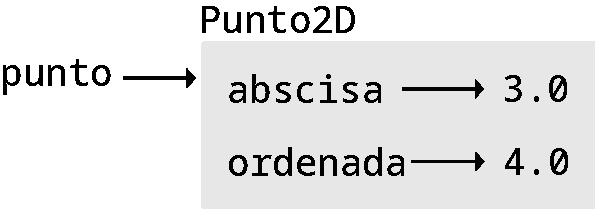
\includegraphics[scale=0.8]{figs/point2D.pdf}}
\caption{Diagrama de objeto.}
\label{fig.point2d}
\end{figure}

La variable {\tt \$punto} se refiere a un objeto {\tt Punto2D},
el cual contiene dos atributos. 

Cada atributo de la clase {\tt Punto2D} debe referirse a un 
número, pero esto no es obvio en la definición actual de la clase.
Al momento podemos crear un objeto {\tt Punto2D} con un cadena de texto
como la abscisa, lo cual no hace sentido. Podemos mejora la definición de
la clase al especificar un tipo numérico para los atributos:
%
\begin{lstlisting}
class Punto2D {
	has Numeric $.abscisa;               # valor "x"
	has Numeroc $.ordenada;              # valor "y" 
}
\end{lstlisting}
%
\index{private attribute}
\index{attribute!private}
Los atributos de la instancia son privados para la clase,
lo cual significa que no puede accederse fuera de la clase:
usualmente necesitarías invocar un método de la clase (i.e., un
tipo de subrutina definida dentro de la clase), para obtener su
valor. No obstante, cuando se define un atributo con un punto como 
en \verb|$.abscisa|:

\begin{lstlisting}
    has $.abscisa;  
\end{lstlisting}
%
\index{accessor}
\index{method!accessor}
Perl crea un método implícito \emph{de acceso}, i.e., un método
que comparte el nombre del atributo y devuelve el valor de dicho
atributo. Así que, cuando escribimos:

\begin{lstlisting}
say $punto.abscisa;                     # -> 3
\end{lstlisting}
%
no estábamos accediendo el atributo {\tt abscisa} del objeto
\verb|$punto| directamente, sino que estábamos llamando al método
{\tt abscisa} sobre el objeto, el cual devolvió el valor de ese
atributo.

\index{dot notation}
\index{accessor}

Puedes usar dicho un método de acceso con la notación de punto
como parte de cualquier expresión. Por ejemplo:

\begin{lstlisting}
my $dist-al-centro = sqrt($punto.abscisa ** 2 + $punto.ordenada ** 2);
\end{lstlisting}
%

También hay otra manera de declarar un atributo en una clase, 
usando el twigil de signo de exclamación en vez de un punto:
\index{twigil}

\begin{lstlisting}
    has $!abscisa;  
\end{lstlisting}
%
\index{attribute!private}
\index{private attribute}
En ese caso, Perl no crea un método implícito de acceso 
y el atributo solo se puede acceder desde otros métodos
dentro de la clase. Tal atributo es ahora completamente privado. 
Sin embargo, si declaras atributos de esta manera, no podrás
asignarles ningún valor durante la creación del objeto con el 
constructor por defecto {\tt new} y necesitarás crear tu propio
constructor (or modificar {\tt new} indirectamente). Así que no
intentes esto por el tiempo presente, dado que no serás capaz
de hacer mucho con tus objetos en este punto. Regresaremos a esto 
más tarde.

\index{attribute!mutable}
\index{attribute!immutable}
Por defecto, los atributos de un objeto no son mutables; solo
se pueden leer. Esto significa que no puedes modificarlos una vez que 
se ha creado el objeto. Esto funciona bien para algunos atributos: si
un objeto representa a una persona, es poco probable que el nombre 
de la persona y su fecha de nacimiento cambien. Otros atributos necesitan
ser actualizados, muchas veces muy frecuentemente. En tales casos, los
atributos pueden declararse como mutables con el rasgo (del inglés \emph{trait})
 {\tt is rw}:
\index{is rw trait}
\index{trait!is rw}

\begin{lstlisting}
class Punto2D {
	has Numeric $.abscisa is rw;               # valor "x"
	has Numeroc $.ordenada is rw;              # valor "y" 
}
\end{lstlisting}
%
Ahora es posible modificar estos atributos. Por ejemplo,
podemos cambiar la abscisa del punto recién creado:

\begin{lstlisting}
# Primero creamos un objeto Punto2D:
my $punto = Punto2D.new(abscisa => 3, ordenada => 4);
say $punto;    # -> Punto2D.new(abscisa => 3, ordenada => 4)

# Ahora movemos el objeto $punto dos unidades a la derecha:
$punto.abscisa = 5; 
say $punto;    # -> Punto2D.new(abscisa => 5, ordenada => 4)
\end{lstlisting}


\index{class!attribute}
\index{attribute!class}
Casi toda la información presentada aquí acerca de los atributos
está relacionada con los atributos de la instancia, i.e., propiedades
relacionada a objetos individuales. También puedes tener atributos que
pertenecen a la clase entera, los cuales se conocen como \emph{atributos de la
clase}. Son menos común que los atributos de una instancia y son declarados
con el declarador {\tt my} (en vez de {\tt has}). Un ejemplo típico de
una atributo de una clase sería un contador al nivel de la clase para
mantener un récord del número de objetos que se han instanciado.


\section{Creando Métodos}
\index{method}

La simple clase {\tt Punto2D} y su instancia \verb|$punto|
no son muy útil al momento. Completemos la definición de la
clase con algunos métodos:
\index{Point2D class}

\begin{lstlisting}
class Punto2D {
    has Numeric $.abscisa;
    has Numeric $.ordenada;
    
    method coordenadas {        #  método de acceso para "x" y "y"
        return (self.abscisa, self.ordenada)
    }
    
    method distancia-al-centro {
        (self.abscisa ** 2 + self.ordenada ** 2) ** 0.5
    }
    method coordenadas-polares {
        my $radio = self.distancia-al-centro;
        my $theta = atan2 self.ordenada, self.abscisa;
        return $radio, $theta;
    }
}
\end{lstlisting}

Aquí declaramos tres métodos en la clase:
\begin{itemize}
\item {\tt coordenadas}, un simple método de acceso a
las coordenadas cartesianas;
\index{coordinates!Cartesian}
\index{Cartesian coordinates}

\item{\tt distancia-al-centro}, un método que calcula y devuelve
la distancia entre el objeto y el origen;

\index{polar coordinates}
\index{coordinates!polar}
\item{\tt coordenadas-polares}, un método que calcula el radio y 
el azimuth (\verb|$theta|) del objeto en el sistema de coordenada
polar (nota que {\tt coordenadas-polares} invoca al método 
{\tt distancia-al-centro} para encontrar el componente radio de las 
coordenadas polares).
\end{itemize}

\index{invocant}
La definición de un método no es muy distinta a la definición
de una subrutina, excepto que usa la palabra clave {\tt method}
en vez de {\tt sub}. Esto no es una sorpresa dado que un 
método es esencialmente una subrutina que se define dentro de
una clase (o un rol) y sabe acerca de su \emph{invocante}, i.e.,
el objeto que lo llama y su clase. Y, por supuesto, tiene una
sintaxis de llamada diferente.
\index{method}

\index{method!dispatch}
\index{dispatching methods}
\index{invocation!method}
\index{method invocation}
Otra diferencia importante entre una subrutina y un método es
que, debido a que hay varios métodos con el mismo nombre
definidos en diferentes clases (o diferentes roles), una 
invocación de método conlleva un fase de \emph{despacho},
en la cual el sistema de objeto selecciona cuál método llamar,
usualmente basado en la clase o tipo del invocante. Sin embargo,
en Perl~6, esa diferencia no es muy clara por hecho de que 
puedes tener multi subrutinas, i.e., subrutinas con el mismo
y una signatura diferente que son resueltas al tiempo de ejecución,
dependiendo en la \emph{aridad} (número de argumentos) y el 
tipo de los argumentos.
\index{arity}
\index{type}

Dentro de la definición de un método, {\tt self}
se refiere al \emph{invocante}, el objeto que invocó
al método. Existe un atajo para el mismo, \verb|$.|,
así que podríamos escribir el método {\tt coordenadas}
de la siguiente manera:
\index{self}

\begin{lstlisting}
    method coordenadas {        #  método de acceso para "x" y "y"
        return ($.abscisa, $.ordenada)
    }
\end{lstlisting}

Los dos formatos de sintaxis, \verb|$.| y {\tt self}, son
esencialmente equivalentes.

Existe una tercera manera de lograr el mismo objetivo,
la cual usa el signo de exclamación en vez del punto:

\begin{lstlisting}
    method coordenadas {        #  método de acceso para "x" y "y"
		return ($!abscisa, $!ordenada)
	}
\end{lstlisting}

Aquí, el resultado sería el mismo, pero esta nueva sintaxis
no es equivalente: \verb|$.abscisa| es una invocación de método,
mientras que \verb|$!abscisa| provee acceso directo al atributo. 
La diferencia es que \verb|$!abscisa| está disponible dentro de 
la clase (y podría ser un poco más rápida), mientras
la sintaxis de invocación de método puede ser usada en cualquier
otra parte (por ejemplo dentro de otra clase). Veremos en la 
siguiente sección ejemplos de esta distinción y sus consecuencias.
\index{invocation!method}
\index{method invocation}

Podemos ahora crear un objeto e invocar nuestros métodos:

\begin{lstlisting}
my $punto =  Punto2D.new(
    abscisa => 4, 
    ordenada => 3
);
say $punto.coordenadas;            # -> (4 3)
say $punto.distancia-al-centro;    # -> 5
say $punto.coordenadas-polares;    # -> (5 0.643501108793284)
\end{lstlisting}

\index{topical variable}
\index{invocant}
Podría ser que recuerdes que si usas un método sin nombrar el
invocante explícitamente, entonces el método se aplica
a la \verb|variable tópico|:

\begin{lstlisting}
.say for <one two three>;       # -> one two three (cada uno en su propia línea)
\end{lstlisting}

\index{for loop}
\index{given statement}
Ahora que hemos creado un objeto con algunos métodos, también
podemos tomar ventaja de la misma sintaxis. Por ejemplo, si 
usamos {\tt for} o {\tt given} para poblar la variable tópico
\verb|$_| con el objeto \verb|$punto|, podemos escribir:

\begin{lstlisting}
given $punto {
    say .coordenadas;             # -> (4 3)                       
    say .distancia-al-centro;     # -> 5                 
    .coordenadas-polares.say;     # -> (5 0.643501108793284)
}    
\end{lstlisting}

Como ejercicio, podrías escribir una subrutina llamado 
\verb|distancia-entre-puntos| que toma dos puntos
como argumentos y devuelve la distancia entre ellos 
usando el teorema de Teorema de Pitágoras.

Los métodos de nuestra clase son todos métodos de acceso,
lo cual significa que ellos proveen el estado de algunos de los atributos
del invocante. Si los atributos son mutable (al ser declarados con
con el trait \verb|is rw|), podemos también creamos algunos \emph{mutadores},
i.e., métodos que se invocan para cambiar aquellos atributos mutables:
\index{accessor}
\index{mutator}

\begin{lstlisting}
class Punto2D-mutable {
    has Numeric $.abscisa is rw;
    has Numeric $.ordenada is rw;
    
    # quizás los mismos métodos de acceso como
    # en la clase anterior.
    
    method nueva-ordenada (Numeric $ord) {
        self.ordenada= $ord; 
    }
}
# Creando un objeto Punto2D-mutable:
my $punto = Punto2D-mutable.new(abscisa => 3, ordenada => 4);
say $punto;  # -> Punto2D-mutable.new(abscisa => 3, ordenada => 4)

# Modificando la ordenada:
$punto.nueva-ordenada(6);
say $punto;  # -> Punto2D-mutable.new(abscisa => 3, ordenada => 6)
\end{lstlisting}




\section{Rectángulos y Composición de Objetos}
\label{rectangles}
\index{rectangle}
\index{composition!object}
\index{object!composition}

Algunas veces es obvio qué los atributos de un objeto deberían ser,
pero otras veces debes hacer decisiones. Por ejemplo, imagínate que estás
diseñando una clase para representar rectángulos. ?`Qué atributos usarías para
especificar la ubicación y tamaño de un rectángulo? Puedes ignorar 
los ángulos; para mantener las cosas simples, asume que los bordes 
del rectángulo son verticales or horizontales.
\index{representation}

Existen por lo menos dos posibilidades:

\begin{itemize}

\item Podrías especificar una esquina del rectángulo (o el centro), 
el ancho, y la altura.

\item Podrías dos esquinas opuestas.

\end{itemize}

En este momento es difícil decir cuál de las opciones es mejor, 
así que implementaremos la primera, como un ejemplo.
\index{Rectangle class}
\index{class!Rectangle}

Aquí está la definición de la clase:

\begin{lstlisting}
class Rectángulo {
    has Numeric $.ancho;
    has Numeric $.altura;
    has Punto2D $.esquina;     # vértice inferior izquierdo 

    method area { return $.ancho * $.altura }
    method superior-izq { $.esquina.abscisa, $.esquina.ordenada + $.altura; }
    # otros métodos, e.g. para las coordenadas de las otras esquinas,
    # centro, etc.
}
\end{lstlisting}
%
La nueva característica comparada a la definición 
anterior de la clase {\tt Punto2D} es que la clase 
\verb|Rectángulo| ahora usa el tipo {\tt Punto2D} 
creado anteriormente para definir el atributo esquina.

El método {\tt superior-izq} devuelve las coordenadas 
del ángulo superior izquierdo del rectángulo. Este 
método {\tt superior-izq} nos da la oportunidad de explicar
un poco más acerca de la diferencia entre los twigils
\verb|$.| y \verb|$!|. Hemos usado \verb|$.esquina.abscisa|
para obtener la abscisa de la esquina, i.e., en efecto una
invocación del método de acceso. Podríamos haber accedido 
los atributos {\tt esquina} y {\tt altura} de la clase
{\tt Rectángulo} directamente y usar la siguiente definición
de método:
\index{twigil}
\index{invoother methodscation!method}
\index{method invocation}

\begin{lstlisting}
    method superior-izq { 
    	$!esquina.abscisa, $!esquina.ordenada + $!altura;
    }
\end{lstlisting}

Sin embargo, no sería posible \verb|$!esquina!abscisa| o 
\verb|$.esquina!abscisa|, dado que {\tt abscisa} no es un 
atributo definido en la clase {\tt Rectńgulo}, y por lo tanto
no se puede acceder directamente ahí. Puedes usar acceso directo
del atributo (por ejemplo con la sintaxis \verb|$!abscisa|)
solo dentro de la clase donde el atributo es definido, {\tt Punto2D}.
Así que, en {\tt Rectángulo}, necesitamos invocar el método de
acceso (i.e., la sintaxis con \verb|$.|) para obtener el valor
de abscisa de la esquina. 

Ahora podemos crear un objeto {\tt Rectángulo}:
\index{rectangle}

\begin{lstlisting}
my $punto-inicio =  Punto2D.new(abscisa => 4, ordenada => 3);
my $rect = Rectángulo.new(
	esquina => $punto-inicio, 
	altura => 10, 
	ancho => 5
);

say "Coord. de esquina superior-izq.: ", $rect.top-left;   
			# -> Coord. de esquina superior-izq.: (4 13)
say "Area del rectángulo: ", $rect.area;      
			# -> Area del rectángulo: 50
\end{lstlisting}


\index{named parameter}
\index{parameter!named}
Podrás haber notado que los argumentos que pasan al 
constructor {\tt Rectángulo.new} no están en el mismo 
orden como en la definición de la clase. Hice eso a 
propósito para mostrar que el orden de los argumentos
no importan porque estamos usando argumentos nombrados.

La figura~\ref{fig.rectangle} muestra el estado de este objeto.

\begin{figure}
\centerline
{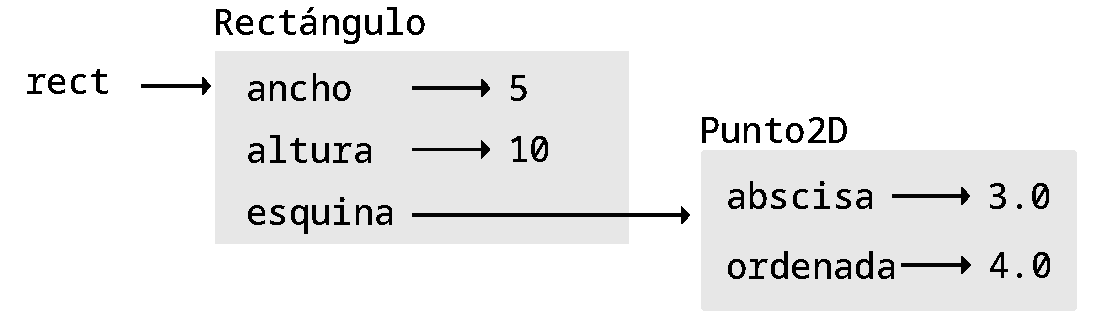
\includegraphics[scale=0.7]{figs/rectangle.pdf}}
\caption{Diagrama de objeto.}
\label{fig.rectangle}
\end{figure}

\index{state diagram}
\index{diagram!state}
\index{object diagram}
\index{diagram!object}
\index{embedded object}
\index{object!embedded}
\index{object!composition}
\index{composition!object}

El uso de un objeto como un atributo de otro objeto, posiblemente
de otra clase, se conoce como {\bf composición de objeto}. 
Un objeto que es un atributo de otro objeto es un objeto 
{\bf embebido}. La composición de objeto hace posible 
definir capas anidadas de abstracción y es una característica
poderosa de la programación orientada a objetos. En nuestro 
ejemplo de ``geometría``, comenzamos a definir un objeto 
a un nivel inferior, una instancia {\tt Punto2D}, y después usamos
ese punto para construir un tipo a un nivel superior, {\tt Rectángulo}.


\section{Instancias como Valores de Retorno}
\index{instance!as return value}
\index{return!value}

Los métodos pueden devolver instancias de otras clase. 
Por ejemplo, la clase {\tt Rectángulo} puede tener métodos
de devuelven instancias de {\tt Punto2D} para las otras
esquinas:

\begin{lstlisting}
    method punto-superior-der {
        return Punto2D.new(
            abscisa  => $!esquina.abscisa + $!ancho, 
            ordenada => $!esquina.ordenada + $!altura
        );
    }
   # otros métodos para las otras esquinas
\end{lstlisting}

Nota que no tenemos que molestarnos en darle un nombre al
punto superior derecho (aunque podríamos si quisiéramos);
podemos crearlo con el constructor y devolverlo inmediatamente.

Podemos usar el nuevo método como sigue:

\begin{lstlisting}
my $puntoSupDer = $rect.punto-superior-der;
say "Esquina superior derecha: ", $puntoSupDer;
# -> Esquina superior derecha: Punto2D.new(abscisa => 9, ordenada => 13)
\end{lstlisting}

\index{type}
Aunque esto no es muy útil en casos simples como este, 
podríamos asegurarnos y declarar un tipo {\tt Punto2D}
para \verb|$puntoSupDer|:

\begin{lstlisting}
my Punto2D $puntoSupDer = $rect.punto-superior-der;
\end{lstlisting} 

De este modo, el código levantará un error si {\tt punto-superior-der}
devuelve algo más que una instancia {\tt Punto2D}.

Similarmente, el método \verb|encontrar-centro| invocado 
sobre un {\tt Rectángulo} devuelve una instancia de 
{\tt Punto2D} que representa el centro del {\tt Rectángulo}:

\begin{lstlisting}
    method encontrar-centro { Punto2D.new(
            abscisa  => $!esquina.abscisa  + $!ancho / 2, 
            ordenada => $!esquina.ordenada + $!altura / 2
        );
    }
\end{lstlisting}
%
Este nuevo método puede ser usado en la siguiente manera:

\begin{lstlisting}
say "Centro = ", $rect.encontrar-centro;
# -> Centro = Punto2D.new(abscisa => 6.5, ordenada => 8.0)
\end{lstlisting}
%

\section{Herencia}
\index{inheritance}
\index{inheritance!class}
\index{class!inheritance}

La herencia es probablemente la característica más 
emblemática de la programación orientada a objetos.
Es un mecanismo a través del cual es posible derivar una
clase de otra clase. La herencia es una de las maneras 
estándares de implementar la reutilización de código en la
programación orientada a objeto. Es también otra manera útil 
de definir capas sucesivas de abstracción y una 
jerarquía de tipos.

\subsection{La Clase Pixel}
\index{class!Pixel}
\index{Pixel class}

La clase {\tt Punto2D} es muy general y podría usarse para
una variedad de propósitos: geometría, gráficas vectoriales, 
mangas animados, etc. Podríamos querer usarlo para mostrar 
datos gráficos en la pantalla. Para este escenario, crearemos
una nueva clase derivada {\tt Pixel}, agregaremos nuevas 
propiedades al punto, tales como color, quizás transparencia, etc.

?`Necesitamos redefinir todos los atributos y los métodos para la 
nueva clase? No, no necesitamos hacer esto. Podemos definir una 
nueva clase que \emph{hereda} las propiedades de la clase base 
{\tt Punto2D} y solo modificamos lo que no es adecuado o agregamos nuevas
características si las necesitamos. Aquí, queremos un nuevo
atributo para representar el color de un píxel y probablemente
algunos otros métodos para manejar este nuevo atributo.

De acuerdo a los estándares más comunes, un color es definido
por tres enteros (realmente tres octetos, i.e., enteros entre 
0 y 255 en la notación decimal), que representan los componentes
rojo, verde y azul de un píxel. Esta combinación de componentes es normalmente
conocida como RGB (sigla en inglés de {\bf R}ed, {\bf G}reen y {\bf B}lue en inglés):
\index{class!child}
\index{Pixel class}
\index{RGB}
\index{octet}

\begin{lstlisting}
class Pixel is Punto2D {
    has %.color is rw;

    method cambiar_color(%tono) {
        %!color = %tono
    }
    method cambiar_color2(Int $rojo, Int $verde, Int $azul) {
        # signatura usando parámetros de posición
        %!color = (rojo => $rojo, verde => $verde, azul => $azul)
    }
}
\end{lstlisting}

\index{parameter!positional}
\index{parameter!named}
\index{positional parameter}
\index{octet}
\index{is!subclassing trait}
La nueva clase \emph{hereda} las propiedades de la {\tt Punto2D}
gracias al rasgo {\tt is Punto2D}, excepto posiblemente
aquellos que son explícitamente modificados (o anulados) o agregados
en la nueva clase. Esta nueva clase es algunas veces llamada
una clase hija o subclase, mientras que {\tt Punto2D} es la
clase padre, clase base o superclase. La creación de esta nueva
clase basada en {\tt Punto2D} se como {\bf subclassing} de la 
clase base {\tt Punto2D}.
\index{class!parent}
\index{class!child}
\index{class!subclass}
\index{subclassing}
\index{overriding a method}
\index{method!overriding}

La nueva clase hija hereda los atributos {\tt abscisa} y 
{\tt ordenada} de la clase padre {\tt Punto2D} (y sus 
propiedades específicas si tienen algunas), al igual que los
métodos tales como {\tt coordenadas} el cual es definido en
la clase padre. La clase hija tiene un nuevo atributo (el color)
y dos métodos nuevos.

Instanciar un objeto {\tt Pixel} es tan fácil como antes,
solo necesitamos agregar un argumento adicional correspondiente
al nuevo atributo cuando invoquemos el constructor {\tt new}:
\begin{lstlisting}
my $pix = Pixel.new(
	:abscisa(3.3),
	:ordenada(4.2),
	color => {rojo => 34, verde => 233, azul => 145}, 
);

say "El píxel original tiene los siguientes colores:", $pix.color;
\end{lstlisting}

In the {\tt Pixel} class definition, we have written 
two different methods for changing the color 
only to illustrate two possible syntax formats, for pedagogical 
purposes.

En la definición de la clase {\tt Pixel}, escribimos dos métodos
diferentes para cambiar el color solo para ilustrar posibles 
formatos de sintaxis, para propósitos pedagógicos. El primer método
recibe un hash como un parámetro, y el segundo usa parámetros de posición,
los cuales forzan al usuario recordar el orden (RGB) en el cual los
argumentos deben pasarse; esto puede ser una fuente de errores y 
debería evitarse cuando el número de parámetros excede un cierto 
límite (lo cual se dejará al lector). Por otro lado, cualquier 
persona que trabaja con gráficas sabe de memoria la convención estándar 
del orden de los colores (i.e., RGB). También, el segundo método
tiene la ventaja de habilitar el chequeo de tipo (los argumentos
deben ser números enteros). Esto es un ejemplo simplificado; en la
vida real, sería deseable chequear si los parámetros son octetos, i.e.,
enteros entre 0 y 255 (lo cual se podría hacer al añadir un
una restricción de tipo o al definir un subconjunto del tipo entero).
\index{subset}
\index{RGB}
\index{octet}

Usar la nueva clase {\tt Pixel} es bien directo:

\begin{lstlisting}
say "Colores originales: ", $pix.color;

$pix.cambiar_color({:rojo(195), :verde(110), :azul(70),});
say "Colores modificados: ", $pix.color;
say "Nuevas características del píxel:";
printf "\tAbscisa: %.2f\n\tOrdenada: %.2f\n\tColores: R: %d, G: %d, B: %d\n",
       $pix.abscisa, $pix.ordenada, 
       $pix.color<rojo>, $pix.color{"verde"}, $pix.color{"azul"};

$pix.cambiar_color2(90, 180, 30);  # argumentos de posición
say "Nuevos colores:  
\tR: {$pix.color<rojo>}, G: {$pix.color<verde>}, B: {$pix.color<azul>} ";
\end{lstlisting}

Esto muestra lo siguiente en la pantalla:

\begin{lstlisting}
Colores originales: {azul => 145, rojo => 34, verde => 233}
Colores modificados: {azul => 70, rojo => 195, verde => 110}
Nuevas características del píxel:
Abscisa: 3.30
Ordenada: 4.20
Colores: R: 195, G: 110, B: 70
Nuevos colores:  
R: 90, G: 180, B: 30 
\end{lstlisting}

Para decir la verdad, no era necesario usar dos métodos con
nombres diferentes, \verb|cambiar_color| y \verb|cambiar_color2|,
como hicimos en la definición de la clase {\tt Pixel} para 
simplificar el asunto. Funcionaría de la misma manera si usáramos
estas definiciones:
\index{Pixel class}
\index{method dispatch}

\begin{lstlisting}
    multi method cambiar_color(%tono) {
        self.color = %tono
    }
    multi method cambiar_color(Int $rojo, Int $verde, Int $azul) {
        # signatura usando parámetros de posición
        self.color = (rojo => $rojo, verde => $verde, azul => $azul)
    }
\end{lstlisting} 

Debido a que el método multi se define dos veces, con el 
mismo nombre pero diferente signatura, el sistema de objeto
es capaz de despachar la invocación al método correcto.
\index{method!dispatch}
\index{multi method}


\subsection{La Clase PuntoMovible}
\index{class!MovablePoint}
\index{MovablePoint class}

Los atributos \verb|$.abscisa| y \verb|$.ordenada| de la 
clase {\tt Punto2D} son por defecto atributos con solo
acceso de lectura. Después de todo, cuando defines un punto
en el plano, usualmente tiene una posición fija y generalmente 
no hay razón para cambiar su coordenada.

Sin embargo, supón que nuestra aplicación es acerca de la
cinemática (la rama de la física que estudia el movimiento
de puntos o cuerpos) o es un videojuego. En tal caso, probablemente
queremos que nuestros puntos (o conjunto de puntos) puedan 
moverse. Necesitamos una nueva clase, {\tt PuntoMovible},
para habilitar la modificación de las coordenadas.

No necesitamos redefinir todos los atributos y métodos para
la nueva clase. Otra vez, podemos definir una nueva clase
que \emph{herede} las propiedades de la clase base {\tt Punto2D}
y solo modifique aquello que no es adecuado o agregue 
nuevas características que necesitemos, por ejemplo:

\begin{lstlisting}
class PuntoMovible is Punto2D {
    has Numeric $.abscisa is rw;
    has Numeric $.ordenada is rw;
    
    method mover (Numeric $x, Numeric $y) {
        $.abscisa  += $x;
        $.ordenada += $y;
    }
}
\end{lstlisting}

\index{is!subclassing trait}
La nueva clase hereda las propiedades de {\tt Punto2D} 
gracias al rasgo {\tt is Punto2D}, excepto que aquellos
que son explícitamente modificados (o anulados) o agregados
en la nueva clase. Los métodos que existen en la clase padre
y se redefinen en la clase hija se dice que son \emph{anulados}
dentro esa clase.
\index{class!parent}
\index{class!child}
\index{class!subclass}
\index{subclassing}
\index{overriding a method}
\index{method!overriding}

Aquí, los atributos \verb|$.abscisa| y \verb|$.ordenada| 
se redefinen con acceso de lectura y escritura (a través del rasgo
{\tt is rw}) y un método nuevo, {\tt mover}, es definido para modificar
la posición de un punto al añadir los parámetros recibidos a las
coordenadas del punto.
\index{is rw trait}

Nota que hemos usado parámetros de posición para el método {\tt mover}. 
Dijimos que es usualmente mejor por motivos de claridad usar parámetros
nombrados, pero hemos usado solo dos parámetros aquí; debido a que 
es bastante simple recordar que el parámetro \verb|$x| debería venir
antes que el parámetro \verb|$y|. Esto fue una ocasión para ilustrar la
posibilidad de usar parámetros de posición.
\index{positional parameter}
\index{parameter!positional}
\index{parameter!named}
\index{named parameter}

Ahora podemos probar nuestra clase hija, crear una instancia 
{\tt PuntoMovible}, mostrar sus características, moverla a una
posición diferente, y mostrar la posición nueva. 

\begin{lstlisting}
my $punto = PuntoMovible.new(
    abscisa => 6,
    ordenada => 7,
    );

say "Coordenadas: ", $punto.coordenadas;
say "Distancia al origen: ", $punto.distancia-al-centro.round(0.01);
printf "%s: radio = %.4f, theta (rad) = %.4f\n", 
    "Coordenadas polares", $punto.coordenadas-polares;

say "--> Moviendo el punto.";
$punto.mover(4, 5);
say "Nuevas coordenadas: ", $punto.coordenadas;
say "Distancia al origen: ", $punto.distancia-al-centro.round(0.01);
printf "%s: radio = %.4f, theta (rad) = %.4f\n", 
    "Coordenadas polares", $punto.coordenadas-polares;
\end{lstlisting}

Esto produce la siguiente salida:

\begin{lstlisting}
Coordenadas: (6 7)
Distancia al origen: 9.22
Coordenadas polares: radio = 9.2195, theta (rad) = 0.8622
--> Moviendo el punto.
Nuevas Coordenadas: (10 12)
Distancia al origen: 15.62
Coordenadas polares: radio = 15.6205, theta (rad) = 0.8761
\end{lstlisting}

\index{polar coordinates}
\index{coordinates!polar}
Aquí, cuando el usuario invoca los métodos {\tt coordenadas},
{\tt distancia-al-centro}, y {\tt coordenadas-polares}, Perl
encuentra que dichos métodos no existen en la clase {\tt PuntoMovible}.
Pero, dado que \verb|PuntoMovible| es una subclase de {\tt Punto2D},
el programa hace una búsqueda de estos nombres en la clase padre, 
y los invoca si los encuentra. Si no los encuentra, entonces podría
buscar en el padre de la clase padre para ver si se encuentran ahí, etc.


\subsection{Herencia Múltiple: Atractiva Pero, es de Sabio Utilizarla?}

En la programación orientada a objeto, el mecanismo de herencia
es una manera tradicional de reutilizar código. Es probablemente 
la forma más común de hacerlo.

Un clase puede tener varias clases padres y, por lo tanto,
ser una subclase de otras clases. Esto es lo que se conoce como
{\bf herencia múltiple}. Podríamos construir una nueva 
clase {\tt PixelMovible} la cual hereda de {\tt PuntoMovible} 
y de {\tt Pixel} (e, indirectamente, de {\tt Punto2D}). Técnicamente,
puedes hacer esto fácilmente en Perl:

\begin{lstlisting}
class PixelMovible is PuntoMovible is Pixel {
    # ...
}
\end{lstlisting}

Ahora, {\tt PixelMovible} es una clase de {\tt PuntoMovible}
y {\tt Pixel} y hereda de ambas clases padres.
\index{subclass}
\index{class!parent}

Esto luce bastante prometedor, pero sucede que tiende a ser
más complicado de lo esperado en situaciones reales. Si existe
un conflicto (por ejemplo una colisión de nombre entre dos método),
cuál debe prevalecer? Algunos mecanismo existen para manejar tales
situaciones (por ejemplo en el lenguaje de programación C++), y
Perl tiene métodos metaobjetos para encontrar información
sobre el orden de resolución de los métodos (MRO por sus siglas en inglés),
pero esto puede rápidamente conducir a varios problemas de diseño y a
errores (\emph{bugs}) que son sutiles y complicados. En resumen, 
mientra la herencia múltiple originalmente lucía como una atractiva idea, 
resultó ser en algo muy complicado de dominar,
porque crea dependencias múltiples, y usualmente implícitas, que son 
difíciles de arreglar.

Esta es la razón por la cual, contrario a C++, relativamente reciente lenguajes de programación orientados a objetos como Java (el cual surgió no tan recientemente, en 1995) han decidido no implementar herencia múltiple.

Perl~6 no quiere prohibir tales cosas y como resultado te permite
hacer uso de la herencia múltiple si deseas, la cual puede ser 
muy útil para casos simples. Así que no la descarte innecesariamente,
pero recuerdas que, contrario a las expectaciones originales, 
la herencia múltiple usualmente conduce a un desastre y resulta
ser incontrolable.

Perl ofrece mejores conceptos para encargarse de tales situaciones, como
veremos en un momento.

\section{Roles y Composición}
\index{role}
\index{inheritance}

La herencia es un concepto poderoso para describir un árbol jerárquico de
conceptos. Por ejemplo, puedes pensar de una jerarquía de figuras geométricas
que tienen una o más propiedades específicas: 
\begin{enumerate}
\item Polígono

\index{quadrilateral}
\item Cuadrilátero (un polígono con cuatro lados y cuatro esquinas)

\index{trapezoid}
\item Trapezoide (un cuadrilátero con un par de lados paralelos)

\index{parallelogram}
\item Paralelogramo (un trapezoide con dos pares de lados paralelos y lados
opuestos de la misma longitud)

\index{rectangle}
\item Rectángulo (un paralelogramo con cuatro ángulos rectos)

\index{square}
\item Cuadrado (un rectángulo con cuatro lados iguales)
\end{enumerate}

\index{rhombus}
Es relativamente fácil de imaginar una serie de clases con un árbol de
herencia jerárquica que refleje esas propiedades. Se vuelve más 
complicado, sin embargo, si agregamos el rombo (un paralelogramo con
todos los lados iguales), porque el cuadrado es ahora \emph{también}
un rombo con cuatro ángulos rectos. La clase cuadrado sería una 
subclase del rectángulo y del rombo, y podríamos tener un posible
caso de herencia múltiple.

\index{integer} \index{rational} \index{real number} \index{complex number}
\index{vertebrate} \index{mammal} \index{carnivoran}
\index{canid} \index{dog}
Similarmente, podemos pensar acerca de un árbol de clases con herencia
anidada que representan varios tipos de números (e.g., entero, 
racional, real, complejo) o especies de animales (e.g., vertebrado, 
mamífero, carnívoro, canino, perro, setter irlandés).

\index{hierarchical model}
Estos son ejemplos grandiosos de herencia, pero el mundo real es
raramente jerárquico, y es usualmente difícil de forzar cada caso 
a encajar en un modelo jerárquico.

\index{role}
Esta es una de la razones por la cual Perl introduce la noción
de roles. Un rol es un conjunto de comportamientos o acciones
que pueden compartirse entre varias clases. Técnicamente, un rol
es una colección de métodos (posiblemente con algunos atributos);
es por lo tanto similar a una clase, pero la primera diferencia
obvia es que un rol no está diseñado para ser instanciado como
un objeto (aunque los roles pueden ser promovidos al estado de
clases). La segunda diferencia, quizás la más importante, es que los
roles no heredan: ellos se usan al ser aplicados a una clase 
o/y una composición.

\subsection{Clases y Roles: Un Ejemplo}

\index{vertebrate} \index{mammal} \index{dog}
Volvamos con los vertebrados, mamíferos y perros. Un perro
es un mamífero y hereda algunas características de los 
mamíferos tales como una neocórtex (una región del cerebro),
pelo, y glándulas mamarias, también como una columna vertebral,
la cual todos los mamíferos (incluyendo los peces, aves, reptiles, etc.)
heredan de los vertebrados. Hasta ahora, la jerarquía de la clase
parece simple y natural.

\index{feral animal}
\index{pet animal}
No obstante los perros pueden tener diferentes características y
comportamientos. Para citar un artículo de Wikipedia sobre los perros:
``Los perros tienen un sin número de \emph{roles} para las personas
entre los que figuran la caza, el pastoreo, halar cargas pesadas, asistir
a la policía y el ejército, compañía y, recientemente, asistir a
individuos incapacitados`` (énfasis añadido). Los perros también pueden 
ser animales salvajes (i.e, animales que viven en ambientes silvestres
pero que han descendido de individuos domesticados) o perros callejeros.
Todos comportamientos adicionales pueden añadirse a la clase perro.
Similarmente, un gato, otro mamífero, puede ser una mascota o
un animal salvaje. Los mustangos, caballos salvajes de Norteámerica,
también son animales salvajes, descendientes en algún tiempo de caballos
domesticados; pero un mustango puede capturarse y puesto devuelta
en un estado domesticado. Este retorno a lo salvaje de animales
silvestres no está limitado a los mamíferos: las palomas que viven
en nuestras ciudades descendieron una vez de palomas mensajeras
usadas en el pasado. Puede hasta ocurrir con invertebrados, tales
como enjambres de abejas melíferas.

Es aparente que un modelo jerárquico de arboles de herencia
no está adaptado para describir tales comportamientos.

\index{vertebrate} \index{mammal} \index{dog}
Podemos definir clases para los perros, los gatos, y los 
caballos como subclases de mamíferos (los cuales también heredan
de los vertebrados). Además de eso, podemos definir roles para mascotas
o animales salvajes. En adición, podemos crear nuevas clases
que son subclases de las clases perro, gato y caballo y que 
tienen algunos roles específicos. Del mismo modo, podemos
asignar roles a instancias individuales de una clase. Esto
podría lucir así (este un ejemplo ficticio que no se puede probar):

\begin{lstlisting}
class Vertebrado { method hablar {say "vertebrado"};}
class Mamífero is Vertebrado  { method hablar { say "mamífero" } }
class Ave      is Vertebrado  { method volar     {} }
class Perro    is Mamífero    { method ladrar    {} }
class Caballo  is Mamífero    { method relinchar {} }
class Gato     is Mamífero    { method maullar   {} }
class Ratón    is Mamífero    { method chillar   {} }
class Pato     is Ave         { method graznar   {} }
# ...

role Animal-mascota { 
    method es-compañero() {...} 
    # otros métodos
}
role Ovejero     { ... }    # pastor de ovejas
role Salvaje     { ... }    # animal en un ambiente salvaje
role Guía        { ... }    # guía de los ciegos
role Humano-comp { ... }    # animal que se comporta como un humano
# ...

class Perro-guía          is Perro   does Guía           { ... }
class Perro-ovejero       is Perro   does Ovejero        { ... }
class Perro-callejero     is Perro   does Salvaje        { ... }
class Gato-mascota        is Gato    does Animal-mascota { ... }
class Gato-salvaje        is Gato    does Salvaje        { ... }
class Mustago             is Caballo does Salvaje        { ... }
class Canario-dom         is Ave 	 does Animal-mascota { ... }
# ...
# Un rol se puede aplicar a instancias:
my $garfield = Gato-mascota.new(...);
my $mickey   = Ratón.new(...);
$mickey does Humano-comp;
my $donald   = Pato.new(...);
$donald does Humano-comp; 
my $pluto    = Perro.new(...);
$pluto does Animal-mascota;
my $snoopy   = Perro.new(...);
$snoopy does Animal-mascota does Humano-comp;
\end{lstlisting}
 
\index{role!application}
\index{does trait}
\index{trait!does}
\index{trait!is}
Un rol se aplica a una clase o a un objeto con el rasgo
{\tt does} (opuesto a {\tt is} para la herencia). Estas dos
palabras claves diferentes reflejan la diferencia semántica
asociada con ellas: componer un rol en una clase u objeto
provee dicha clase u objeto con el \emph{comportamiento suplementario}
asociado con el rol, pero esto no significa que al objeto
recibir el rol es la \emph{misma cosa} o de la misma naturaleza como 
el rol.

\index{feral animal}
\index{pet animal}
Si los roles {\tt Animal-mascota} y {\tt Salvaje} hubiesen sido 
definidos como clase, entonces las clases {\tt Gato-mascota} y
{\tt Gato-salvaje} hubiesen experimentado herencia doble,
con los problemas potenciales asociados con eso. Al aplicar
un rol a una clase, evitas construir un árbol de herencia múltiple
que probablemente no se puede justificar y que puede ser difícil de
conceptualizar y manejar. Un uso juicioso de clases y roles puede 
conducir a un modelo que es más simple, más natural, y más cercano
a las relaciones reales entre las entidades y comportamientos 
bajo escrutinio.

\index{multiple inheritance}
\index{method!dispatch}
\index{role!composition}

In adición, si compones varios roles inadvertidamente con dos
métodos que poseen el mismo nombre, esto inmediatamente levanta
un error (a menos que un método con el mismo nombre exista dentro
de la clase y en tal caso, prevalece), en lugar de despachar silenciosamente
a una de los métodos como en el caso de herencia múltiple. En 
ese caso, los conflictos de nombre son identificados inmediatamente
(al tiempo de compilación), lo cual tiene el beneficio de 
encontrar un error inmediatamente, el cual podría no ser
perceptible por un largo tiempo.

\subsection{Composición de un Rol y Reutilización de Código}

Las clases son para manejar instancias y los roles son para
manejar comportamientos y reutilización de código. El siguiente
ejemplo muestra cómo las clases y los roles funcionan bien juntos.
\index{class}
\index{role}
\index{code reuse}

\begin{lstlisting}
role Dibujable {
    has $.color is rw;
    method dibujar { ... }
}
class Figura {
    method area { ... }
}
class Rectángulo is Figura does Dibujable {
    has $.ancho;
    has $.altura;
    method area {
        $!ancho * $!ancho;
    }
    method dibujar() {
        for 1..$.altura {
            say 'x' x $.ancho;
        }
    }
}
Rectángulo.new(ancho => 10, altura => 4).dibujar;
\end{lstlisting}

\index{ellipsis}
Ten presente que la intención de los puntos suspensivos
\verb|...| usados en el código anterior es representar
código que se deja para tu implementación. Sin embargo, esto
es actualmente código válido y se compilará y hasta se 
ejecutará sin ningún problema. Los puntos suspensivos 
son usados para representar una funcionalidad que no se ha
implementado todavía pero que se hará en el futuro. Esto funcionará
siempre y cuando to no invoques estos métodos (lo que producirá un 
error de ejecución) o crees una situación donde ellos necesitarían
estar definidos (lo que ocasionará un error de compilación).
En el caso del método {\tt dibujar} en el role {\tt Dibujable},
la composición de rol en la clase {\tt Rectángulo} funciona
solo porque {\tt dibujar} es redefinido en la clase {\tt Rectángulo};
sin esta redefinición, hubiese levantado un error al tiempo de
compilación. Similarmente, el código \verb|method area { ... }|
de la clase {\tt Figura} levantaría un error al tiempo de
ejecución si fuera llamado sin haber sido redefinido en
la clase {\tt Rectángulo}. Los puntos suspensivos se han usado 
aquí como una manera conveniente de representar código cuyo 
implementación no es importante para nuestro ejemplo porque se está
redefiniendo de cualquier modo. En código real, es probablemente
recomendado no usar puntos suspensivos, excepto como expediente temporario
para código que no se ha desarrollado todavía pero que será
implementado.

El código de más arriba dibuja un rectángulo ASCII:
\begin{lstlisting}
~ perl6 test_drawable.pl6
xxxxxxxxxx
xxxxxxxxxx
xxxxxxxxxx
xxxxxxxxxx
\end{lstlisting}

\subsection{Roles, Clases, Objetos, y Tipos}
\index{role}
\index{class}
\index{object}
\index{type}

Un rol se puede aplicar a una clase entera o solamente a 
algunas instancias de la clase:

\begin{lstlisting}
role Guía { ...}
class Perro-guía is Perro does Guía { 
    ... 
}  # Componiendo el rol Guía en la clase Perro-guía
   # la cual hereda de la clase Perro

my $perrito = new Perro; # creando un objeto Perro
$doggy does Guide;       # aplicando el rol al objeto
\end{lstlisting}

\index{type}
\index{role!type}
\index{type!-defining role}
\index{guide}
Los roles y las clases son diferentes, pero ambos son tipos
o definen tipos. Esto significa que un rol puede usarse como
un tipo para una declaración de variable donde esperaría el 
nombre de una clase. Por ejemplo, el rol {\tt Guía} en el fragmento
de código anterior efectivamente crea un tipo {\tt Guía}. Así que
un rol {\tt Invidente} para un humano podría tener un atributo
de tipo {\tt Guía}, el cual representaría un perro-guía, un 
caballo-guía, un humano-guía o hasta un robot-guía.

\begin{lstlisting}
class Humano {
    has Perro $perro;  # Puede contener cualquier perro,
    		  # con o sin un rol guía
}
role Invidente {
    has Guía $guía;  # Puede contener un tipo Guía, 
    	  	# un perro, un caballo, un humano, o un robot
}
\end{lstlisting}

\index{type!built-in}

Una mayoría de los tipos integrados de Perl~6 son definidos
por roles y no clases, tales como {\tt IO}, {\tt Iterable}, 
{\tt Iterator}, {\tt Numeric}, {\tt Rational}, {\tt Real},
etc.

\section{Delegación de Método}
\index{delegation}


La {\bf Delegación} es otra manera de enlazar un objeto a otra pieza 
de código. La técnica de delegación ha sido estudia extensivamente 
al nivel teórico e implementada en algunos cuantos lenguajes 
especializados de investigación, pero la implementación de
delegación en los lenguajes generalistas convencionales
es bien inusual.

En lugar de definir métodos en una clase o en un rol, la idea 
es invocar los métodos perteneciente a otro objeto, como si fueran
métodos de la clase actual. En Perl~6, la delegación puede realizarse
al nivel de una clase o un rol. Un objeto delegado es simplemente
un atributo definido en una clase o en un rol con la palabra clave
{\tt handles} que posibilita especificar cuales métodos del objeto 
delegado pueden ser usados en la clase actual:

\index{Cervantes, Miguel de} \index{Shakespeare, William} 
\index{Chekhov, Anton} \index{Schiller, Friedrich} \index{Hamlet} 
\index{Don-Quijote} \index{Don-Carlos} \index{Three Sisters}
\begin{lstlisting}
class ClaseBase {
    method Don-Quijote()    { "Cervantes"   }
    method Hamlet()         { "Shakespeare" }
    method Three-Sisters () { "Chekhov"     }
    method Don-Carlos()     { "Schiller"    }
}

class Uses { 
    has $.base is rw handles < Don-Quijote Hamlet Three-Sisters >;
}

my $user = Uses.new;
$user.base = ClaseBase.new(); # implementando un object-handler
say $user.Don-Quijote;
say $user.Hamlet;
say $user.Three-Sisters;
say $user.Don-Carlos;
\end{lstlisting}

Esto muestra lo siguiente:

\begin{lstlisting}
Cervantes
Shakespeare
Chekhov
Method 'Don-Carlos' not found for invocant of class 'Uses'
  in block <unit> at delegate.pl6 line 16
\end{lstlisting}
\index{invocant}

El programa muestra apropiadamente los nombres de los
escritores que los primeros tres métodos devuelve, porque ellos
han sido más o menos ``importados`` en la clase {\tt Uses}, pero 
falla con el último, porque ``Don-Carlos`` no es parte de la 
lista del handler. El error en el último método es una excepción al
tiempo de ejecución y el programa terminaría la ejecución ahí aún
hubiera algún código correcto después. 

Nota que la clase {\tt Uses} no sabe de donde los métodos 
serán importados; solo sabe sobre los nombres de los 
métodos que serán importados. Solamente cuando el objeto
\verb|$user| es creado y el atributo \verb|$user.base|
es añadido, el objeto es dinámicamente con los métodos
definidos en {\tt ClaseBase}. Casualmente, este proceso
puede hacerse en un solo paso:

\begin{lstlisting}
my $user = Uses.new( base => ClaseBase.new() );
\end{lstlisting}

No hay necesidad de enumerar los métodos que serán manipulados.
La clase {\tt Uses} puede importar todos los métodos de 
{\tt ClaseBase}:

\begin{lstlisting}
class Uses { 
    has $.base is rw handles ClaseBase;
}
\end{lstlisting}

Esto funcionará como antes, excepto que no fallará con el método
{\tt Don-Carlos} ahora, debido a que este método fue importado también:

\begin{lstlisting}
Cervantes
Shakespeare
Chekhov
Schiller
\end{lstlisting} 

\section{Polimorfismo}
\index{polymorphism}
\index{interface}

El polimorfismo es una manera de suplir un interfaz común o 
relacionada a tipos diferentes. En cierta manera, los ejemplos
de herencia que estudiamos anteriormente ofrecen una forma
de polimorfismo: los métodos {\tt coordenadas}, {\tt distancia-al-centro}, y {\tt coordenadas-polares} son polimórficos, debido a que ellos pueden aplicar a los tipos
{\tt Punto2D}, {\tt PuntoMovible} y {\tt Pixel}. Hablaremos de
polimorfismo cuando los métodos relevantes o funciones hacen cada uno algo diferente, por lo menos al nivel de implementación, aún
compartan el mismo nombre y misma interfaz.

\index{multi!subroutine}
\index{invocant}
Fuera de la programación orientada a objeto (POO), las subrutinas
\emph{multi} de Perl implementan una forma de polimorfismo,
dado que se comportan de forma diferente dependiendo del tipo
y número de sus argumentos. Dentro del contexto POO, es
usualmente el tipo del invocante (su clase o posiblemente uno de
sus roles) que determinará, usualmente al tiempo de 
ejecución, cuales de los posibles métodos será invocado.

Por ejemplo, podríamos querer crear una nueva clase para 
puntos en el espacio tridimensional. Los métodos tendrán 
que ser diferentes, pero sería interesante ofrecer al usuario
un interfaz que es igual (o casi igual)  a aquella de los
puntos en dos dimensiones:
\index{Point3D class}

\begin{lstlisting}
class Punto3D {
    has Numeric $.x;
    has Numeric $.y;
    has Numeric $.z;
    
    method coordenadas () {      # método de acceso a las 3 coordenadas
    	return $.x, $.y, $.z
    }
    method distancia-al-centro () {
        return ($.x ** 2 + $.y ** 2 + $.z ** 2) ** 0.5
    }
    method coordenadas-polares () {
    	return self.coordenadas-esféricas;
    }
    method coordenadas-esféricas {
    	my $rho = $.distance2center;
    	my $longitud = atan2 $.y, $.x;          # theta
    	my $latitud = acos $.z / $rho;          # phi 
    	return $rho, $longitud, $latitud;
    }
    method coordenadas-cilíndricas {
    	# ...
    }
}
\end{lstlisting}

Los métodos en esta nueva clase no son los mismos que 
en {\tt Punto2D}, pero los métodos con semánticas similares
tienen el mismo nombre; así que es posible usar cualquiera
de las clases sin perderse con nombres diferentes.

El método {\tt distancia-al-centro} tiene exactamente la misma interfaz. El método {\tt coordenadas} devuelve una lista de tres 
valores en lugar de dos, pero la convención de llamada es la misma. Nota que podría haber sido posible diseñar {\tt Punto2D}
de tal manera que este método devolviera un tercer valor cero, 
para tener exactamente la misma interfaz (después de todo, un punto en el plano podría ser considerado como un punto en el 
espacio 3D con altura cero); cumplir exactamente con la misma
interfaz no es mandatorio, pero solo una posible implementación
que podría hacer una interfaz más intuitiva.
 

\index{polar coordinates}
\index{spherical coordinates}
\index{coordinates!polar}
\index{coordinates!spherical}
La noción de coordenadas polares no tiene un significado 
bien definido en el espacio 3D, pero he elegido mantener el nombre
en nuestra interfaz porque es intuitivamente similar a la idea
de coordenadas esféricas; no hace nada más que invocar 
el método \verb|coordenadas-esféricas| sobre su invocante y
devolver los valores de retorno.
\index{invocant}

Por favor nota que los matemáticos, físicos, astrónomos, ingenieros, geógrafos, y navegadores todos usan el mismo sistema
básico para las coordenadas esféricas, pero sus convenciones
son diferentes con respecto al origen, rango del ángulo, 
unidades medidas de ángulos y dirección de rotación, y el nombre de los varios valores o símbolos asociados con los mismos. 
Así que podrías encontrar diferentes fórmulas en un libro de
texto. Las convenciones y fórmulas que hemos usado son comúnmente
utilizadas en geografía y algunas ramas de las matemáticas. Una clase real de propósito general tendría que tomar en cuenta toda estas convenciones e implementar las convenciones necesarias.

\section{Encapsulación}

\index{encapsulation}
La encapsulación es la idea de ocultar los datos y código 
de una librería o un módulo del usuario. El concepto no es
específico a la programación orientada a objeto, pero 
es parte fundamental de la misma.

\index{accessor}
\index{mutator}
\index{getter}
\index{setter}
En la programación orientada a objetos, la encapsulación 
consiste de proteger los datos en un objeto de manipulación
directa (y de manera inconsistente) por el usuario, quien 
acceder tales datos a través de los métodos. Esto se logra al
proveer al usuario métodos que son conocidos como \emph{métodos 
de acceso} (o \emph{getters}) y \emph{mutadores} (o \emph{setters}).
Esto hace posible asegurar que las propiedades del objeto 
serán validadas por sus métodos. 


\index{black box}
\index{object!interface}
La encapsulación es una forma poderosa de abstracción
y abstracción procedimental. Visto desde afuera, un
objeto es una caja negra que tiene propiedades y 
comportamientos específicos. De esta forma, estas propiedades
y comportamientos están \emph{ocultos} del usuario. 
No están ocultos en el sentido de que el usuario no puede
saber sobre ellos (por lo menos en el mundo de código 
abierto (\emph{open source}), es fácil saber esto), pero
que están ocultos en el sentido de que es usualmente no posible
usar ese conocimiento para eludir la interfaz proveída.
Esto significa que la implementación interna del objeto 
puede cambiar sin tener que modificar el comportamiento
externo. Si usas conocimiento privilegiado, tu código
probablemente no funcionará correctamente cuando la 
implementación interna sea modificada. Por lo tanto,
no hagas eso.

Varios lenguajes de programación no tienen las mismas reglas para
garantizar encapsulación. Algunos son más estrictos que otros,
algunos son menos estrictos sobre el acceso de lectura que el
acceso de escritura, otros no hacen tal distinción pero más bien
dependen en el nivel de visibilidad especificado por un atributo,
por ejemplo ``public`` o ``private`` (algunas veces con un nivel 
intermedio ``protegido``).

\index{attribute!private}
Perl~6 te permite eligir el modelo de encapsulación que quieres
aplicar a tus objetos y atributos. Todos los atributos son 
privados. Si declaras una clase así:

\begin{lstlisting}
class Punto2D {
    has $!abscisa;
    has $!ordenada;
    # …
    method valor_x { return $!abscisa }
    method valor_y { return $!ordenada }
}
\end{lstlisting}

las coordenadas \verb|$!abscisa| y \verb|$!ordenada|
serán accesible solo dentro de la clase. Esta es la 
razón por la cual hemos añadido métodos de acceso.
Además, los atributos son inmutables por defecto.

Pero como vimos anteriormente, si declaras
esta clase así:

\begin{lstlisting}
class Punto2D {
    has $.abscisa;
    has $.ordenada;
    # ...
}
\end{lstlisting}

las coordenadas serán todavía atributos privados, pero
Perl~6 generará métodos de acceso automáticamente con los
mismos nombres de los atributos. De esta manera, se pueden
acceder fuera de la clase casi como si fueran públicos:
\index{attribute!public}

\begin{lstlisting}
class Punto2D {
    # ...
}
my $punto = Punto2D.new(abscisa => 2, ordenada => 3);
say $punto.abscisa;       # -> 2
\end{lstlisting}

\index{attribute!mutable}
\index{attribute!immutable}
El rasgo {\tt is rw} maneja separadamente si un atributo 
es mutable o no. En resumen, Perl~6 ofrece un modo acceso por
defecto, pero puedes configurarlo y lo que necesitas.


\subsection{Métodos Privados}
\index{private method}
\index{method!private}
\index{interface}

Los métodos son la manera normal de usar objetos, ya sea con
solo acceso de lectura o con acceso de lectura y escritura. 
Usualmente forman la \emph{interfaz} de una clase, que es la
parte de la clase que es pública y disponible para los programadores que deseen usarla. Es por lo tanto natural y legítimo que los métodos sean públicos, i.e, accesibles fuera
de la clase.
\index{method!public}
\index{public method}

Pero una clase puede también contener numerosos métodos
que son parte de la receta de cocina interna de la clase, i.e.,
la forma en la que hace las cosas internamente, y que no están
destinadas a ser usadas fuera de la clase. Es posible prevenir 
su uso fuera de la clase al hacer estos métodos privados. 
Un método privado de Perl~6 se prefija con un signo de 
exclamación:

\begin{lstlisting}
method !comportamiento-privado($x, $y) {
    ...
}
\end{lstlisting}

También necesitarás usar un signo de exclamación para llamarlos:

\begin{lstlisting}
$mi-objecto!comportamiento-privado($val1, $val2)
\end{lstlisting}

\index{private method}
\index{method!private}
Los métodos privados son realmente internos de una clase 
dada. En particular, ellos no son heredados por las clases hijas.


\subsection{Construir Objetos con Atributos Privados}

Construir objetos con atributos privados trae consigo una
pequeña dificultad. Consideremos el siguiente programa:
\index{private attribute}

\begin{lstlisting}
class Punto3D {
    has $.x;
    has $.y;
    has $!z;
    
    method coord_valores {
        return ($!x, $!y, $!z);
    }
};

my $a = Punto3D.new(x => 23, y => 42, z => 2);
say $_ for $a.coord_valores;
\end{lstlisting}

\index{attribute!private}
\index{attribute!public}
En este ejemplo, hemos declarado a \verb|$.x| y \verb|$.y|
como atributos ``públicos`` (por así decirlo), y a \verb|$!z|
como un atributo verdaderamente privado. La ejecución de 
este código muestra lo siguiente:

\begin{lstlisting}
23
42
(Any)
\end{lstlisting}

?`Qué está sucediendo? Parece que el método \verb|coord_valores|
es incapaz de leer el contenido de \verb|$!z|, dado que 
devuelve un valor indefinido. Este método es definido dentro
de la clase y debería ser capaz de acceder este atributo. De hecho,
\verb|coord_valores| no es el problema, sino que \verb|$!z| no está
definido dentro del objeto, porque no se inicializó apropiadamente
durante la creación del objeto.
\index{new!constructor}
\index{constructor!new}
La culpa yace con el constructor implícito {\tt new} que, por
defecto, inicializa solo los atributos ``públicos``.

\index{submethod}
Aquí la solución más simple es probablemente añadir el 
submétodo {\tt BUILD}  en la definición de la clase.
\index{BUILD submethod}

\index{submethod}
\index{subclass}
\index{type}
Un {\tt submétodo} es un método público de una clase que 
no es heredado por sus clases hijas. Semánticamente, es realmente
equivalente a una subrutina, pero se invoca con una sintaxis 
de método (de ahí su nombre). Los submétodos son especialmente útiles
al realizar las tareas de construir y destruir un objeto que no 
deberían ser heredadas por las subclases, también como para las
tareas que son tan específicas para tipo particular que las clases
derivadas tendrán que seguramente modificarlas.

Inicializar los atributos privados durante la instanciación de un objeto
podría lucir así:

\begin{lstlisting}
class Punto3D {
    has $.x;
    has $.y;
    has $!z;

    submethod BUILD (:$!x, :$!y, :$!z) {
        say "!`Inicialización!";
        $!x := $!x; 
        $!y := $!y; 
        $!z := $!z;
    }
    method coord_valores {
        return ($!x, $!y, $!z);
    }
};

my $a = Punto3D.new(x => 23, y => 42, z => 2);
say $_ for $a.coord_valores;
\end{lstlisting}

El programa ahora funciona como se deseaba y muestra 
todos los atributos:

\begin{lstlisting}
!`Inicialización!
23
42
2
\end{lstlisting}

Esto funciona porque el constructor por defecto {\tt new},
un método definido la superclase suprema {\tt Mu} y heredado
por cualquier clase de Perl~6, llama al submétodo por defecto
{\tt BUILD}. Si redefinimos a {\tt BUILD} en nuestra clase, entonces
reemplazará el submétodo por defecto que {\tt new} llama. Al redefinir
a {\tt BUILD}, forzamos el constructor a tomar en cuenta el
atributo privado que no se usó previamente.

Un poco de simplificación es posible. Dado que los argumentos
que se pasan a una rutina enlazan los argumentos a los parámetros,
un paso de enlace separado es innecesario si los atributos se usan
como parámetros. Por lo tanto, el submétodo {\tt BUILD} en el ejemplo
anterior podría también escribirse tan simple como esto:
\index{BUILD submethod}

\begin{lstlisting}
    submethod BUILD(:$!x, :$!y, :$!z) {
        say "!`Inicialización!";
    }
\end{lstlisting}

\index{overriding a method}
\index{named parameter}
\index{positional parameter}
\index{parameter!named}
\index{parameter!positional}
\index{constructor!new}
\index{new!constructor}

Mientras hablamos de las particularidades de la construcción de un objeto,
nota que debido a que {\tt new} es un método heredado desde la superclase
{\tt Mu}, puedes anularlo si lo prefieres. El constructor por defecto
{\tt new} puede usarse solo con argumentos nombrados. Asumiendo que realmente
quieras parámetros de posición, puedes anular a {\tt new} con tu 
propio método, de esta manera:
\index{new!constructor} 
\index{constructor!new}

\begin{lstlisting}
class Punto2D {
    has Numeric $.abscisa;
    has Numeric $.ordenada;

    method new ($x, $y) {
        self.bless(abscisa => $x, ordenada => $y);
    }
    method coordenadas {        # método de acceso a las coordenadas
        return (self.abscisa, self.ordenada)
    }
    # otros métodos
};

my $punto = Punto2D.new(3, 5);
say $_ for $punto.coordenadas;
\end{lstlisting}

Esto mostrará las dos coordenadas. {\tt bless} es un método
de nivel inferior para la construcción de objetos, heredado
desde {\tt Mu} y llamado automáticamente cuando invocas a {\tt new}
para construir un objeto. Usualmente no necesitas saber sobre 
ese método, excepto cuando quieres escribir tu propio
constructor personalizado.

\index{constructor!custom}
Puedes darle un nombre diferente al constructor, por ejemplo:

\begin{lstlisting}
class Punto2D {
    has Numeric $.abscisa;
    has Numeric $.ordenada;

    method construir ($x, $y) {
        self.bless(abscisa => $x, ordenada => $y);
    }
    method coordenadas {        # método de acceso a las coordenadas
        return (self.abscisa, self.ordenada)
    }
    # otros métodos
};

my $punto = Punto2D.construir(3, 5);
say $_ for $punto.coordenadas;
\end{lstlisting}

Aunque deberías pensar dos veces antes de anular a {\tt new} 
o crear tu propio constructor personalizado con un nombre diferente,
dado que podría hacer más difícil la creación de subclases de la 
clase {\tt Punto2D}.



\section{Interfaz e Implementación}

Una de las metas del diseño orientado a objetos es crear software
más fácil de mantener, lo que significa que mantener el programa
funcionando cuando otras partes del sistema cambia, y modificar el 
programa para satisfacer los requerimientos.
\index{interface}
\index{implementation}
\index{maintainable}
\index{object-oriented design}

Un principio de diseño que ayuda a lograr esa meta es mantener
la interfaz separada de las implementaciones. Para objetos, esto
significa que la interfaz pública de los métodos proveídos por una
clase no debería depender en cómo los atributos son representados.
\index{attribute}

\index{coordinates!Cartesian}
\index{Cartesian coordinates}
\index{polar coordinates}
Por ejemplo, diseñamos una clase {\tt Punto2D} en la cual los
atributos principales eran las coordenadas cartesianas del punto.
Podemos descubrir que, para el propósito de nuestra aplicación,
sería más fácil o más rápido almacenar las coordenadas polares del
punto en los atributos del objeto. Es totalmente posible cambiar
la implementación interna de la clase, y aún así mantener
la misma interfaz. Para hacer esto, necesitamos que el constructor
convierte los parámetros de entrada desde coordenadas cartesianas
a polares, y almacenar las coordenadas polares en el
atributo del objeto. El método {\tt coordenadas-polares} devolvería
los atributos almacenados, mientras que los métodos que 
devuelven las coordenadas cartesianas podrían tener que hacer la 
conversión opuesta (o quizás ser almacenados en atributos privados).
En general, el cambio ser podría hacer con la refactorización  
de la clase {\tt Punto2D}, pero los usuarios de la clase todavía
usarían la misma clase sin notar diferencia alguna.

Después de desplegar una nueva clase, podrías descubrir 
una mejor implementación. Si otras partes del programa están
usando tu clase, podría ser un proceso largo y proclive a errores
cambiar la interfaz.

Pero si diseñaste la interfaz cuidadosamente, puedes cambiar
la implementación sin cambiar la interfaz, lo cual significa que las
otras partes del programa no tienen que cambiar.

\section{Programación Orientada a Objetos: Una Fábula}

\index{tale about OOP}
\index{OOP (object-oriented programming)!a tale}
\index{object-oriented programming (OOP))!a tale}
La mayoría de los libros y tutoriales que enseñan 
la programación orientada a objetos se enfocan en los
aspectos técnicos de POO (como hemos hecho en este capítulo
hasta ahora), y esa es una parte muy importante, pero algunas
veces tienden a descuidar las razones de POO. Dicen 
``cómo``, pero no ``porqué``. Hemos intentado explicar
el ``porqué`` (y posiblemente logramos hacerlo bien), pero
esta sección intenta explicar POO desde de la perspectiva de las
razones y los beneficios de POO, independientemente de 
cualquier consideración técnica, en la forma de una parábola (los ejemplos
e código son solo pseudocódigo y no se pueden compilar, menos
ejecutarse).

\subsection{La Fábula del Pastor} 

\index{shepherd}
Había una vez un pastor que tenía un rebaño de ovejas. 
Su típico día de trabajo era así:

\begin{lstlisting}
$pastor.mover_rebaño($pasto);
$pastor.vigilar_rebaño();
$pastor.mover_rebaño($casa);
\end{lstlisting}

Eventualmente, debido a una venta exitosa de lana, él
expandió sus actividades granjeras y su día se volvió
así:

\begin{lstlisting}
$pastor.mover_rebaño($pasto);
$pastor.vigilar_rebaño();
$pastor.mover_rebaño($casa);
$pastor.otro_tarea_importante();
\end{lstlisting}

Pero ahora el pastor quería dedicar más tiempo a 
\verb|otro_tarea_importante()|, así que él decidió 
emplear un subordinado para hacerse cargo de las tareas
relacionadas con las ovejas. De esta manera, el trabajo
se dividió así:
\index{shepherd-boy}
\index{tale about OOP}

\begin{lstlisting}
$niño-pastor.mover_rebaño($pasto);
$niño-pastor.vigilar_rebaño();
$niño-pastor.mover_rebaño($casa);
$pastor.otro_tarea_importante();
\end{lstlisting}

Esto otorgó más tiempo al pastor para la
\verb|otro_tarea_importante()|, pero desafortunadamente
el \verb|$nino-pastor| tenía la tendencia de gritar lobo.
Como resultado, el pastor tuvo que reemplazarlo con un 
asistente nuevo:

\index{sheep dog}
\index{dog!shepherd}
\begin{lstlisting}
$perro-ovejero.mover_rebaño($pasto);
$perro-ovejero.vigilar_rebaño();
$perro-ovejero.mover_rebaño($casa);
$pastor.otro_tarea_importante();
\end{lstlisting}

El \verb|$perro-ovejero| era más falible y demandaba 
un salario más bajo que el \verb|$niño-pastor|, así que
esto representaba una ganancia para el pastor.

\subsection{La Moraleja}

Podemos aprender varias cosas de esta parábola.

\subsubsection{Delegación}
\index{delegation}

Para manejar complejidad, delega a una entidad confiable, e.g.,
el granjero delegó parte de sus responsabilidades al \verb|$niño-pastor|.

\subsubsection{Encapsulación}
\index{encapsulation}

Indica a los objetos que hacer, en lugar de micro-gestionar, e.g.:

\begin{lstlisting}
$perro-ovejero.vigilar_rebaño();
\end{lstlisting}

como esto:

\begin{lstlisting}
$perro-ovejero.cerebro.tarea.vigilar_rebaño();
\end{lstlisting}

A un nivel superior, no nos importa particularmente
la estructura interna del objeto. Solo nos importa
lo que el objeto puede hacer.

Mientra más se expone la estructura interna de un objeto,
más difícil se vuelve cambiarlo.

\subsubsection{Polimorfismo}
\index{polymorphism}
\verb|$perro-ovejero| y \verb|$niño-pastor| ambos
entienden los mismos comandos, así que el reemplazo
del último con el primero fue más fácil de lo que
hubiese sido por el contrario.
\index{tale about OOP}

\emph{La fábula en esta sección es una adaptación de
un post de ``Arunbear```en el sitio web ``PerlMonks``:
\url{http://www.perlmonks.org/?node_id=1146129}. Gracias
a ``Arunbear`` por autorizarme a reutizarla.}


\section{Depuración de Programas}
\label{perl-debugger}
\index{debugger}
\index{debugger!using a}

Esta sección es sobre un depurador, un programa diseñado para
ayudarte a depurar tus programas. ``?`Qué? Tal herramienta existe,
y me lo dices solo ahora?`` podrías quejarte. Bueno, no es realmente
eso. Un depurador no a realizar tus tareas de depuración; todavía 
tienes que hacer el trabajo investigativo difícil, pero un depurador
puede ayudarte a descubrir la razón por la cual tu programa
no hace lo que crees que debería hacer. O, más bien, por qué lo
que tu programa hace no es lo que quieres que haga.

Los depuradores son similares a personas con una fuerte
personalidad: algunas personas los aman y otras los odian. Usualmente,
las personas que no les gustan los depuradores simplemente
nunca tomaron el tiempo de aprender cómo usarlos, pero existen 
algunos programadores expertos que no les gustan y de quienes 
no podemos sospechar de no intentar seriamente. Si te gustan
o no te gustan los depuradores es probablemente un asunto de
gusto personal, pero ellos pueden proveer una ayuda invaluable, si sabes 
cómo usarlos.

\subsection{El Depurador de Perl~6}

\index{debugger!the Perl~6 debugger}
\index{debugger!launching the}
\index{debugging!using a debugger}
\index{debugging!the Perl 6 debugger}
Rakudo-Perl~6 incluye un depurador interactivo que 
llamas con el comando {\tt perl6-debug} (o, en algunas
instalaciones, {\tt perl6-debug-m}). Puedes ejecutar este 
comando, seguido del nombre del programa a depurarse, como
lo normalmente usaría {\tt perl6} con el nombre del programa
para ejecutarlo. Una palabra de advertencia: puedes ejecutar
el depurador con un programa solo si el programa
compila sin ningún error; el objetivo de un depurador no es encontrar 
errores al tiempo de compilación, sino solo errores de
ejecución o errores semánticos.

Una vez que has ejecutado el depurador, verás algo así:

\begin{lstlisting}
>>> LOADING while_done.pl6
+ while_done.pl6 (1 - 3)
| while True {
|     my $line = prompt "Enter something ('done' for exiting)\n";
|     last if $line eq "done";
>
\end{lstlisting}

\index{prompt}
Esto quiere decir que está cargando el programa \verb|while_done.pl6|,
y muestra las primeras líneas del programa; la última línea al fondo
(``\verb">"'')  es un prompt donde puedes entrar algunos comandos.
El programa para en la primera sentencia que actualmente hace algo y espera
por tu entrada. La línea de código que espera ser ejecutada
es resaltada en un color diferente.

\subsection{Cómo Conseguir Ayuda}

\index{debugger!help}
El primer comando que probablemente quieres ejecutar es ``h``,
el cual mostrará la ayuda del depurador y regresará al 
prompt. Abajo, hemos omitido la mayoría de la salida
para ser breve:

\begin{lstlisting}
> h
<enter>                single step, stepping into any calls
s                      step to next statement, stepping over any calls
so                     step out of the current routine
[...]
q[uit]                 exit the debugger
>
\end{lstlisting}

Toma el tiempo para ejecutar ese comando y lee 
las posibles instrucciones que puedes entrar.
Describiremos las más comunes. Como puedes ver arriba,
solo usas ``q`` o ``quit`` para salir del depurador.

\subsection{Recorriendo el Código}

\index{debugger!running code step by step}
\index{debugger!stepping over subroutines}
\index{debugger!stepping out of subroutines}

La característica principal de un depurador es que
te deja ejecutar un programa paso a paso. Cada vez
que presionas la tecla {\tt Enter}, el programa se
moverá un paso hacia adelante (e.g., una línea de 
código). Entrará en una subrutina si la línea de 
código es una llamada de subrutina, pero puedes pasar 
sobre la llamada de la subrutina al ejecutar el comando
``s`` en el prompt del depurador: esto ejecutará la subrutina
y te colocará en la primera línea de código después de la
llamada de la subrutina (y cualquier llamada anidada de otras
subrutinas)ha finalizado. Si entraste en la subrutina pero ya 
no está interesado en recorrerla, solo entra el comando 
``so`` para salir de ahí.

\index{debugger!accessing variables}
A cualquier punto del proceso, puedes mirar el contenido 
de las variables o hasta métodos sobre ellas. Para ver
una variable, escribe su nombre y después presiona 
{\tt Enter}:

\begin{lstlisting}
> $line
"foo"
\end{lstlisting}

También puedes mirar un array o un hash, o usar el
índice o la llave, por ejemplo \verb|@array[10]| o
\verb|%hash{"bar"}|, para visualizar un elemento específico
del array o del hash.

De igual modo, puedes utilizar ``s`` (o ``say``) o ``p`` (o ``print``)
para evaluar y mostrar una expresión en el ámbito actual.

\subsection{Parando en el Lugar Correcto con Puntos de Interrupción}
\index{breakpoint}
\index{debugger!breakpoint}

Podría encontrarlo tedioso recorrer el programa paso a paso
hasta que llegas a la parte interesante. Como sucede, 
tu puedes llegar ahí inmediatamente usando un \emph{punto de
interrupción} (\emph{breakpoint}). Para agregar un punto de 
interrupción, escribe {\tt bp add línea}, donde {\tt línea} es
el número de línea donde quieres que el programa pare 
la ejecución y vuelva de nuevo a recorrer el código línea a 
línea. Después entra el comando ``r`` y el programa se ejecutará
hasta que alcance uno de los puntos de interrupción que has creado.
La ejecución también parará si el programa llega a una excepción;
en ese caso, puedes todavía acceder las variables para intentar 
descubrir lo que pasó. Si no alcanza ningún punto de interrupción
o una excepción, se ejecutará hasta el final.

Puedes ver todos los puntos de interrupción ({\tt bp list}),
remover un punto de interrupción ({\tt bp rm line}), o
remover todos los puntos de interrupción ({\tt bp rm all}).
También puedes crear un punto de interrupción en otro 
archivo (por ejemplo si estás usando un módulo) 
al usar la siguiente sintaxis: {\tt bp add archivo:línea},
donde ``archivo`` es el nombre del archivo.

\subsubsection{Ya Estás Listo para Usar el Depurador}

Probablemente ya sabes lo suficiente para hacer buen uso del 
depurador de Perl~6, recorrer tu programa y descubrir 
donde hace algo que no está supuesto hacer. No fue tanto
que aprender, cierto? !`Inténtalo!

Aún discutiremos varios puntos adicionales.

\subsection{Registrar Información con Puntos de Trace}

\index{debugger!trace point}
Es posible crear puntos de trace en líneas específicas de código y
variables (o expresiones), con el comando {\tt tp add line \$var}.
Esto registrará el valor de \verb|$var| cada vez que el programa
alcanza la línea elegida. Después simplemente ejecutas el 
programa por un momento y, en algún punto, puedes visualizar
cómo la variable cambió a lo largo del tiempo, usando el comando {\tt tp show}.

Por ejemplo, lo usamos para registrar la variable \verb|$palabra-rotada|
en la solución del ejercicio sobre el cifrado César (ver Subsección~\ref{sol_rotate}) 
para la cadena de texto de entrada ``ABCDabcd'' con una rotación
de 25 letras; el comando {\tt tp show} mostró cómo la cadena de texto
codificada fue progresivamente poblada letra por letra:
\index{Caesar cipher}

\begin{lstlisting}
> tp show
>>> rotar.pl6:23
*
* Z
* ZA
* ZAC
* ZACB
* ZACBz
* ZACBza
* ZACBzab
\end{lstlisting}

\subsection{Recorriendo una Coincidencia Regex}
\label{regex-debugging}
\index{regex}
\index{regex!debugging}
\index{debugger!stepping through a regex}

El depurador puede también proveer información útil cuando
el código está intentando coincidir un regex. Por ejemplo, 
supón que ejecutamos un programa con el depurador con el
siguiente código:

\begin{lstlisting}
"foobar" ~~ /f.+b/;
\end{lstlisting}

\index{backtracking}
Si ejecutas el regex paso a paso, la coloración de sintaxis mostrará
átomo por átomo donde está en el regex y que parte de la 
cadena de texto coincide. (No podemos mostrar la coloración de sintaxis
aquí, pero deberías intentarlo para verlo.)

Con el regex arriba, verás que el motor de regex 
intenta coincidir el carácter ``f``del patrón
y encuentra un ``f`` al principio de la cadena de texto;
siguiente, verás que el motor de regex intenta coincidir 
el subpatrón ``+.`` y que coincide la cadena de texto entero;
después, cuando el motor de regex intenta coincidir la 
última ``b`` del patrón, verás que el motor de regex retrocede,
se deshace de la ``r`` y después de la ``a``; finalmente,
el motor de regex tiene éxito con `foob``.
\index{backtracking}

Si tienes dificultad entendiendo cómo los regexes trabajan
o estás mistificado por el retroceso (\emph{backtracking}),
solo ejecuta el depurador sobre algunos regexes y observa
lo que sucede paso a paso. No tienes ni que escribir un 
programa; puedes usarlo en el modo de una sola línea (\emph{one-liner}).
Por ejemplo, para probar el regex de arriba como un one-liner 
en Windows, solo escribe el comando siguiente en el prompt:
\index{one-liner mode}

\begin{lstlisting}
C:\Users\Laurent>perl6-debug-m -e "'foobar' ~~ /f.+b/;"
\end{lstlisting}

Como es usual, cambia las comillas inglesas a comillas simples 
si estás usando cualquier plataforma de Unix.
 
Nuestra nota final sobre el depurador: recuerda siempre entrar
``h`` para conseguir ayuda sobre el comando que necesitas.


\section{Glosario}

\begin{description}

\item[Objeto] Una entidad que encapsula su estado (atributos)
y su comportamiento (métodos).
\index{object}

\item[Clase] Un tipo definido por el programador. La definición de
una clase crea un nuevo tipo de objeto (una forma de abstracción) y
hace posible la instanciación de objetos concretos que representan
datos reales.
\index{class}
\index{programmer-defined type}
\index{type!programmer-defined}

\item[Método] Un tipo especial de subrutina dentro de una clase o un rol,
que puede llamarse usando la sintaxis de la notación del punto.
\index{method}
\index{dot notation}

\item[Objeto de tipo] Un objeto que contiene información sobre un 
tipo definido por el programador. El objeto de tipo puede usarse 
para crear instancias del tipo.
\index{type object}
\index{object!type}

\item[Instancia] Un objeto que pertenece a una clase y contiene
datos reales.
\index{instance}

\item[Instanciar] Crear un nuevo objeto.
\index{instantiate}

\item[Atributo] Una propiedad de estado dentro de la estructura
POO que es similar a una variable. El atributo de una instancia 
es uno de los valores nombrados asociados con un objeto. Los
atributos de una clase son las variable asociadas con la clase
entera. 
\index{attribute!instance}
\index{instance attribute}
\index{attribute!class}
\index{class!attribute}

\item[Objeto integrado] Un objeto que es almacenado como un
atributo de otro objeto.
\index{embedded object}
\index{object!embedded}

\item[Composición de objeto] Uso de un objeto como parte de la 
definición de otro objeto, especialmente el uso de un objeto como
un atributo de otro objeto.
\index{composition}
\index{object!composition}

\item[Diagrama de objeto] Un diagrama que muestra objetos, sus atributos, 
y los valores de dichos atributos.
\index{object diagram}
\index{diagram!object}

\item[Rol] Una colección de métodos similar a una clase pero
que no está diseñada para construir objetos. Un rol contiene 
métodos que pueden aplicarse a una clase o a un objeto para
añadir comportamientos a ellos.
\index{role}

\item[Polimórfico] Perteneciente a una función que funciona con
más de un tipo.  
\index{polymorphism}

\item[Encapsulación] El principio que dicta como la interfaz proveída por un objeto
no debería depender en su implementación, en particular 
la representación de sus atributos. Esto también se conoce como
\emph{ocultación de información}.
\index{encapsulation}
\index{information hiding}

\item[Herencia] La habilidad de crear una nueva clase la cual
es una versión modificada de otra clase previamente definida.
\index{inheritance}

\item[Clase padre] La clase desde la cual la clase hija 
hereda. También conocida como \emph{superclase} o \emph{clase base}.
\index{parent class}

\item[Clase hija] Una nueva clase que hereda de una clase existente;
también llamada \emph{subclase}.
\index{child class}
\index{class!child}

\item[Subclassing] El proceso de crear una clase hija derivada
de una clase padre.
\index{subclass}

\item[Anular] Cuando un método de una clase padre 
es redefinido en una clase hija, se dice que ha sido 
anulado dentro de la clase hija.

\item[Herencia múltiple] Una situación en la cual una clase hija
es derivada y hereda desde más de una clase padre.

\item[Delegación] Definir una clase o un rol en el cual 
es posible invocar métodos que pertenecen a otro objeto.
\index{delegation}

\end{description}

